\documentclass[11pt]{article}
\usepackage[margin=1in]{geometry}
\usepackage{amsmath,amssymb}
\usepackage{graphicx}
\usepackage{booktabs}
\usepackage{siunitx}
\usepackage{xcolor}
\usepackage{caption}
\usepackage[colorlinks=true,linkcolor=blue,citecolor=blue,urlcolor=blue]{hyperref}
\graphicspath{{../output/figures/}}

% ---- result macros (single place to update from output/results/) -----------
\newcommand{\Pexact}{877{,}868}     % P2 exact optimum
\newcommand{\Pnopen}{109}           % P2 substations built
\newcommand{\Pga}{888{,}504}        % P2 GA best
\newcommand{\Psa}{888{,}504}        % P2 SA best
\newcommand{\Ppso}{1{,}024{,}250}   % P2 PSO best
\newcommand{\Pgagap}{1.21}          % P2 GA/SA gap %
\newcommand{\Ppsogap}{16.67}        % P2 PSO gap %
\newcommand{\PoneRedExact}{2{,}874{,}111}  % P1 reduced exact optimum (enumeration)
\newcommand{\PoneRedMILP}{3{,}032{,}631}   % P1 reduced MILP incumbent (CBC stalls)
\newcommand{\PoneFullSA}{4{,}928{,}976}    % P1 full best (SA)
\newcommand{\PoneFullGA}{5{,}038{,}900}    % P1 full best (GA)
\newcommand{\PoneRedMILPgap}{5.52}         % MILP % above true optimum
\newcommand{\Pthreecoi}{40{,}480{,}413}   % P3 COI optimal travel
\newcommand{\Pthreesave}{27.3}      % P3 % saving vs random
% ---------------------------------------------------------------------------

\title{\textbf{Facility and Infrastructure Optimization\\ for a Renewable-Energy Company}\\
\large Exact Mixed-Integer Programming versus Metaheuristics on Three Operations-Research Problems}
\author{Syed Abbas Ahmad}
\date{2026}

\begin{document}
\maketitle

\begin{abstract}
We study three classic operations-research problems arising from a single
renewable-energy company dataset: (P1) laying out 30 departments across 197
candidate sites as a Quadratic Assignment Problem; (P2) siting electrical
substations across 137 demand zones as a Capacitated Facility Location Problem;
and (P3) assigning 20 products to 25{,}189 storage slots to minimize
material-handling travel. Each problem is solved both \emph{exactly} (mixed-integer
or linear programming with the CBC solver via PuLP) and with \emph{metaheuristics}
(genetic algorithm, simulated annealing, particle-swarm optimization), and the
approaches are compared on solution quality, runtime, and optimality gap. The
exact solvers provide provably-optimal baselines where tractable; the
metaheuristics recover near-optimal solutions at scale, with simulated annealing
and the genetic algorithm reaching within \Pgagap\% of optimality on the
substation problem while particle-swarm trails at \Ppsogap\%. For storage, the
Cube-per-Order-Index rule is shown to be provably optimal and to save
\Pthreesave\% of travel over a random layout.
\end{abstract}

\section{Introduction}
The dataset (\texttt{Group 1.xlsx}) describes a renewable-energy company whose
facilities include turbines, photovoltaic maintenance centers, grid-connection
points, substations, and battery storage. It encodes three independent decision
problems that map cleanly onto canonical OR formulations. Our goals are
(i)~rigorous, reproducible models; (ii)~provably-optimal baselines where
tractable; and (iii)~an honest comparison of exact and heuristic methods. We pair exact
mixed-integer and linear programming (PuLP~\cite{mitchell2011pulp} with the CBC
solver~\cite{forrest2005cbc}) with three metaheuristics: a genetic
algorithm~\cite{goldberg1989genetic}, simulated
annealing~\cite{kirkpatrick1983optimization}, and particle-swarm
optimization~\cite{kennedy1995particle}. All code, data, and logged results
accompany this report; every figure and number is regenerated from
\texttt{output/results/} by seeded scripts.

\section{Data}
The data comprises a $30\times30$ asymmetric department flow matrix; 197 candidate
locations with coordinates and a type label; 137 demand zones with electricity
demand, construction cost, capacity, and a $137\times137$ (asymmetric) distance
matrix with forbidden links; and 20 products with throughput and storage
requirements. Parsing, validation, and export are handled by
\texttt{data/loader.py}. Modeling assumptions, including a unit inconsistency in
the substation data that renders the literal reading infeasible, are documented
in \texttt{docs/formulations.md} (assumptions A1--A8) and summarized in
Section~\ref{sec:assumptions}.

\section{P1 -- Department Layout (QAP)}
\subsection{Model}
Assign departments $\mathcal{D}$ to candidate locations $\mathcal{L}$ to minimize
total weighted flow$\times$distance --- the Koopmans--Beckmann quadratic
assignment problem~\cite{koopmans1957assignment,lawler1963quadratic},
\[
\min \sum_{i,j\in\mathcal{D}}\sum_{k,\ell\in\mathcal{L}} f_{ij}\,d_{k\ell}\,x_{ik}x_{j\ell},
\quad \sum_k x_{ik}=1\ \forall i,\quad \sum_i x_{ik}\le 1\ \forall k,
\]
with optional type-compatibility $x_{ik}\le a_{ik}$. Distances are Euclidean from
the site coordinates. Because $|\mathcal{L}|=197>|\mathcal{D}|=30$, this is a QAP
with location selection.

\subsection{Methods and results}
The full instance is intractable exactly ($O(|\mathcal{D}|^2|\mathcal{L}|^2)$
linearization terms), so we obtain the optimum of a reduced $8\times8$ instance by
full enumeration (\PoneRedExact); both the GA and SA recover it exactly. Notably,
a generic McCormick-linearized MILP solved with CBC \emph{stalls} on the same
instance, returning \PoneRedMILP{} ($\approx\PoneRedMILPgap\%$ above the true
optimum) while reporting status ``optimal'' --- a concrete reminder that the QAP
defeats general-purpose branch-and-cut even at small size~\cite{burkard1998qaplib}. On the full
$30\to197$ problem the metaheuristics run alone: simulated annealing reaches
\PoneFullSA{} and the genetic algorithm \PoneFullGA{}, SA outperforming GA as
expected for QAP-type problems. Figure~\ref{fig:p1} shows the resulting layout
and convergence.

\begin{figure}[ht]
\centering
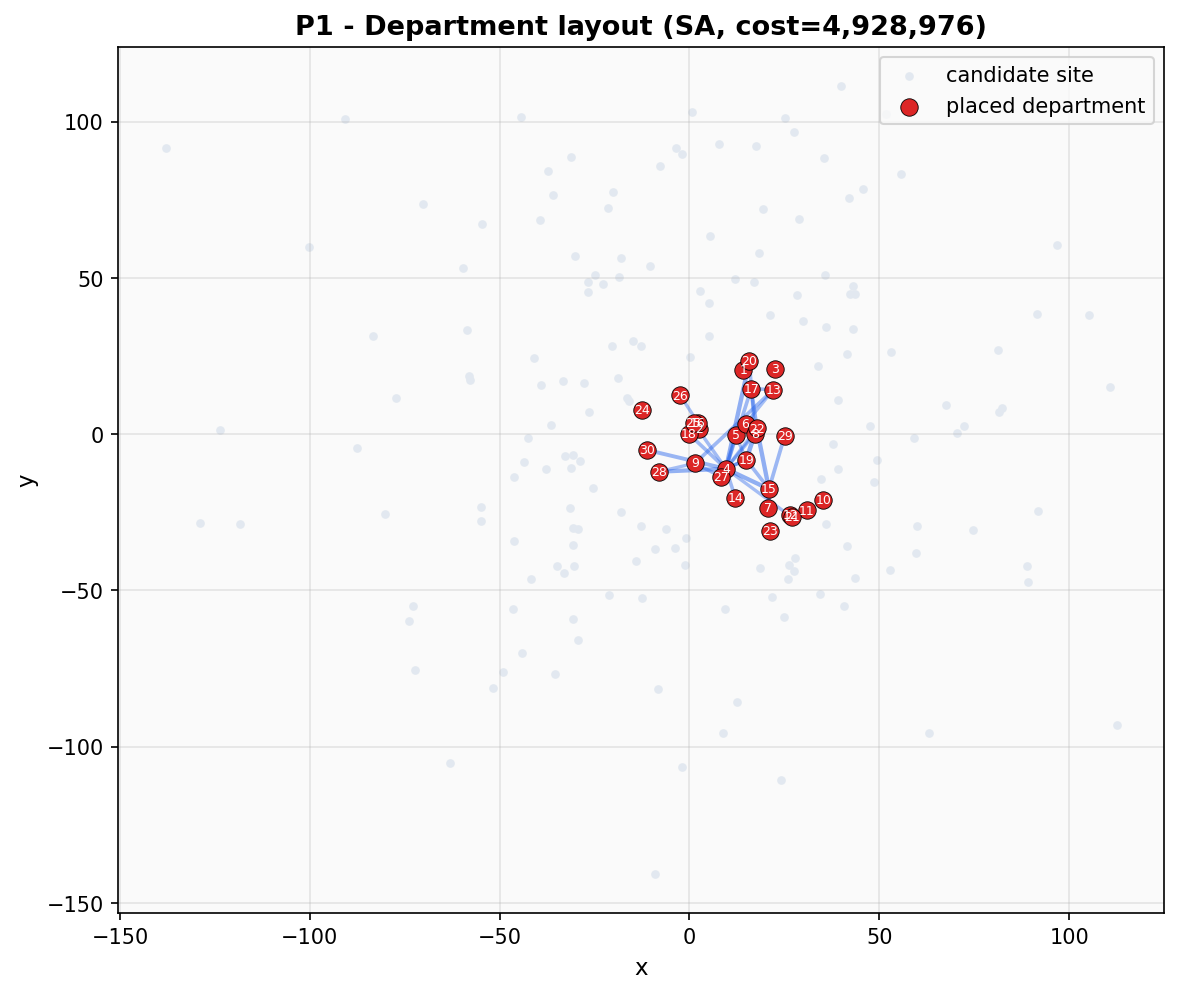
\includegraphics[width=0.62\textwidth]{p1_layout.png}\\
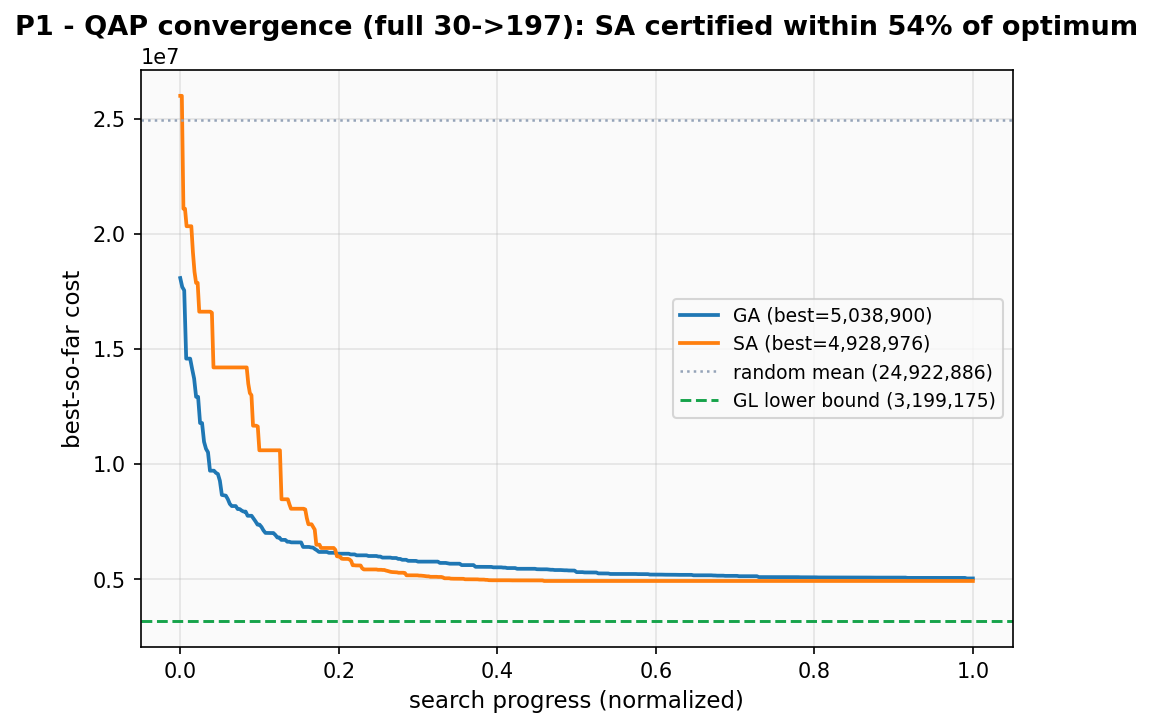
\includegraphics[width=0.62\textwidth]{p1_convergence.png}
\caption{P1: best department layout (top) with high-flow pairs drawn as ribbons,
and GA-vs-SA convergence on the full instance (bottom).}
\label{fig:p1}
\end{figure}

\section{P2 -- Substation Siting (CFLP)}
\subsection{Model}
Open substations and assign zones to minimize construction plus transmission cost
--- a capacitated facility-location problem~\cite{balinski1965integer,daskin2013network},
\[
\min \sum_s c_s y_s + \alpha\sum_{z,s} d_{zs} q_z x_{zs},\quad
\sum_s x_{zs}=1,\ x_{zs}\le y_s,\ \sum_z q_z x_{zs}\le \kappa_s y_s,
\]
single-source, with forbidden links omitted and a self-service diagonal
($d_{ss}=0$). The transmission rate $\alpha$ is calibrated from the data so that
construction and transmission are comparable.

\subsection{Methods and results}
CBC solves the 137-zone instance to optimality (objective \Pexact, \Pnopen{}
substations built). The metaheuristics, run across 10 seeds, give best objectives
of \Pga{} (GA), \Psa{} (SA), and \Ppso{} (PSO), i.e.\ gaps of \Pgagap\% (GA/SA)
and \Ppsogap\% (PSO) to optimality. Particle-swarm, designed for continuous
spaces, is the weakest on this binary problem even with a sigmoid decoding. An
$\alpha$-sweep (Figure~\ref{fig:p2sweep}) traces the classic facility-location
trade-off: as the transmission rate rises, the optimal number of substations
increases and transmission cost falls.

\begin{figure}[ht]
\centering
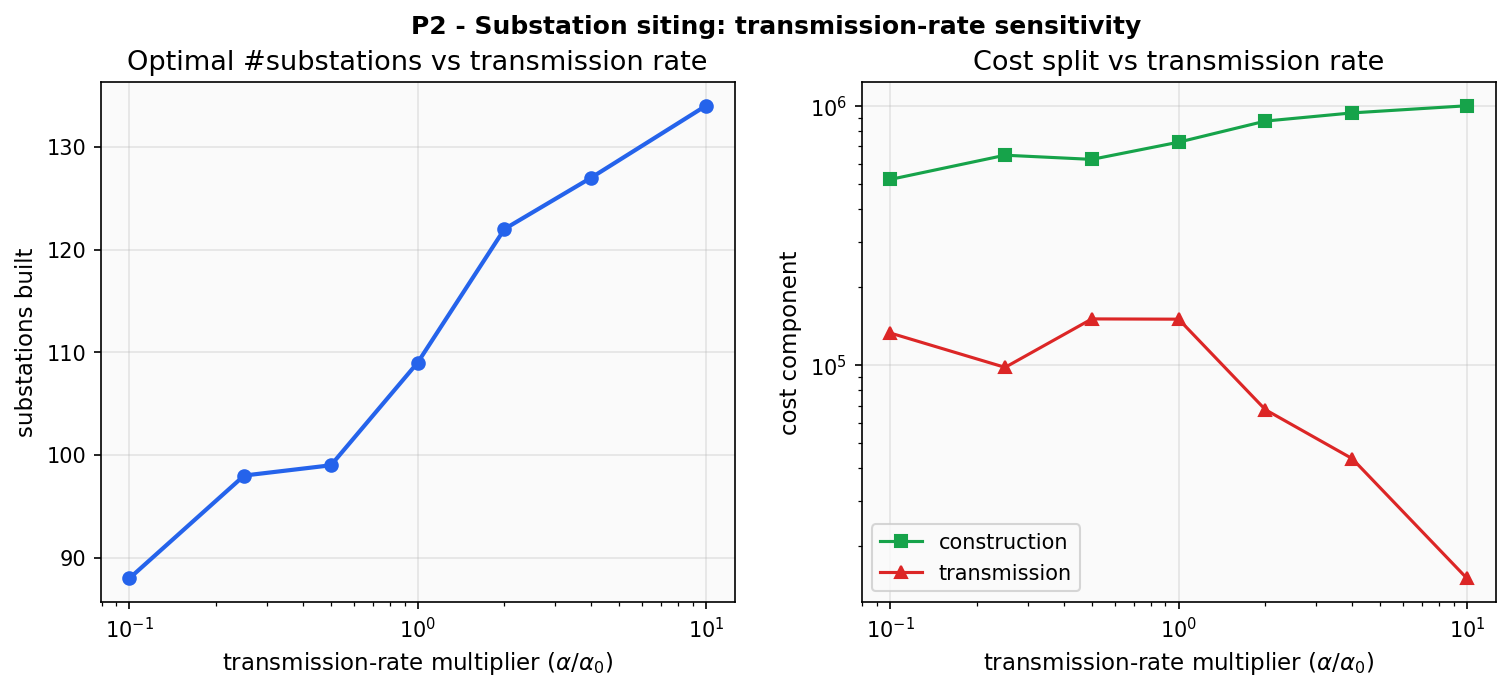
\includegraphics[width=0.92\textwidth]{p2_alpha_sweep.png}
\caption{P2: optimal number of substations and the construction/transmission cost
split as a function of the transmission rate $\alpha$.}
\label{fig:p2sweep}
\end{figure}

\begin{figure}[ht]
\centering
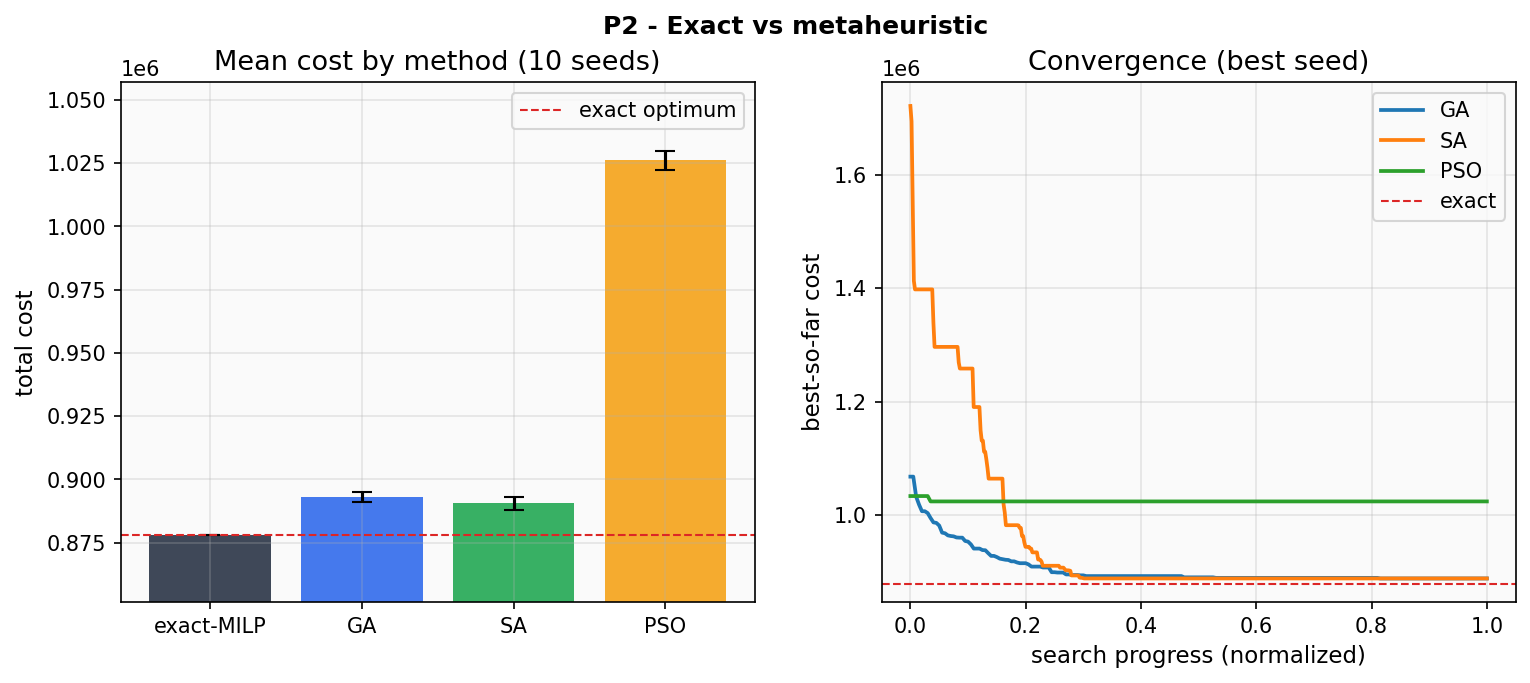
\includegraphics[width=0.92\textwidth]{p2_method_comparison.png}\\
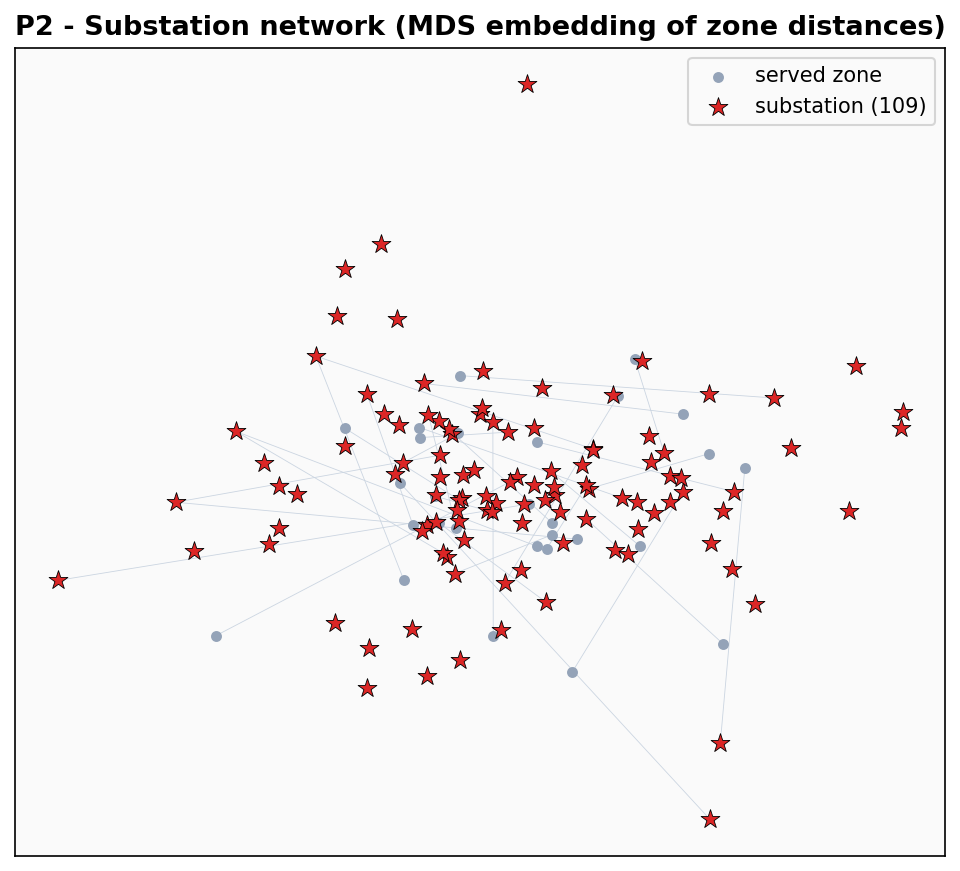
\includegraphics[width=0.55\textwidth]{p2_network.png}
\caption{P2: exact-vs-metaheuristic costs and convergence (top), and the chosen
substation network on an MDS embedding of the zone-distance matrix (bottom).}
\label{fig:p2}
\end{figure}

\section{P3 -- Storage Layout (Cube-per-Order Index)}
\subsection{Model}
Assign products to unit-capacity slots to minimize expected travel,
\[
\min \sum_{p}\sum_{s} \frac{t_p}{q_p}\,\delta_s\, x_{ps},\quad
\sum_s x_{ps}=q_p,\ \sum_p x_{ps}\le 1 .
\]
The constraint matrix is totally unimodular, so the LP relaxation is integral and
its optimum equals the Cube-per-Order-Index (COI) ranking
rule~\cite{heskett1963cube,hausman1976optimal}.

\subsection{Methods and results}
The COI ordering yields optimal travel \Pthreecoi{} at full scale. We verify
optimality three independent ways: an exact transportation LP on a downscaled
instance matches the COI value to machine precision, and both GA and SA over the
product ordering reach the same optimum (0.00\% gap). COI saves \Pthreesave\% of
travel relative to a random layout (Figure~\ref{fig:p3}).

\begin{figure}[ht]
\centering
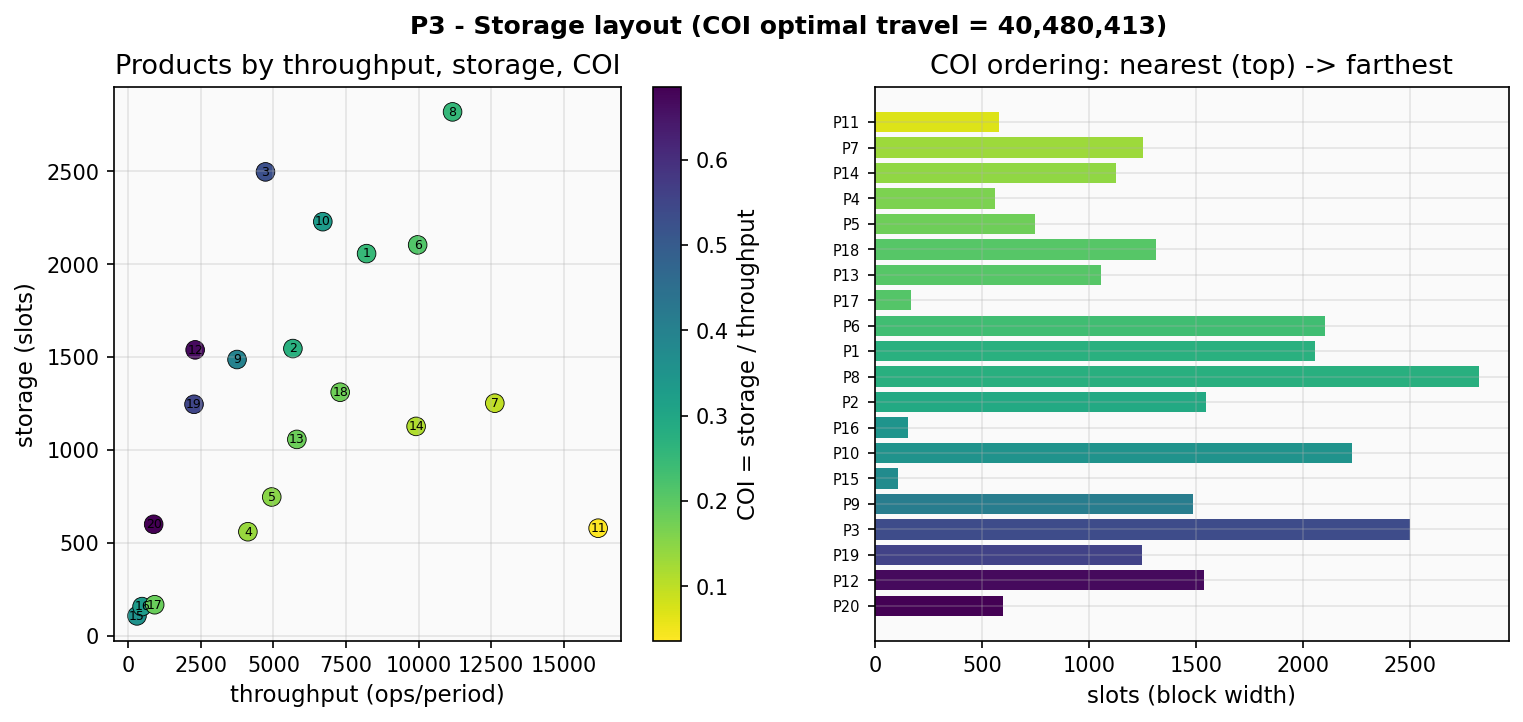
\includegraphics[width=0.92\textwidth]{p3_storage.png}
\caption{P3: products by throughput, storage, and COI (left), and the optimal
nearest-to-farthest slot allocation (right).}
\label{fig:p3}
\end{figure}

\section{Comparison and Discussion}
Across the three problems, exact methods provide optimal or
provably-optimal-on-reduction baselines, while metaheuristics deliver
near-optimal solutions at full scale. Simulated annealing is the most consistent
heuristic (strong on both QAP and CFLP); the genetic algorithm is competitive on
CFLP and storage but weaker on the full QAP; particle-swarm, being continuous by
design, is the weakest on the binary facility-location problem. For the storage
problem, structure (total unimodularity / the COI theorem) makes an exact
polynomial solution available, and the metaheuristics serve only as confirmation.
The optimality gaps are summarized in \texttt{output/results/comparison.csv}.

\section{Assumptions}
\label{sec:assumptions}
All modeling judgment calls are documented as assumptions A1--A8 in
\texttt{docs/formulations.md}. The most consequential is A5/A8 for P2: the literal
demand/capacity units make the instance infeasible, so raw values are treated in a
common unit and a calibrated transmission rate is introduced to avoid a degenerate
``build-everywhere'' optimum.

\section{Reproducibility}
Every experiment is seeded (\texttt{experiments/config.py}) and writes results to
\texttt{output/results/}. Running \texttt{run\_p1}, \texttt{run\_p2},
\texttt{run\_p3}, then \texttt{experiments.compare} and
\texttt{visualization.plot\_solutions} regenerates all numbers and figures in this
report.

\bibliographystyle{plain}
\bibliography{references}

\end{document}
